\documentclass[border=10pt]{standalone}
\usepackage{tikz}
\usetikzlibrary{shapes.geometric}
\usetikzlibrary{arrows.meta,arrows}
\begin{document}

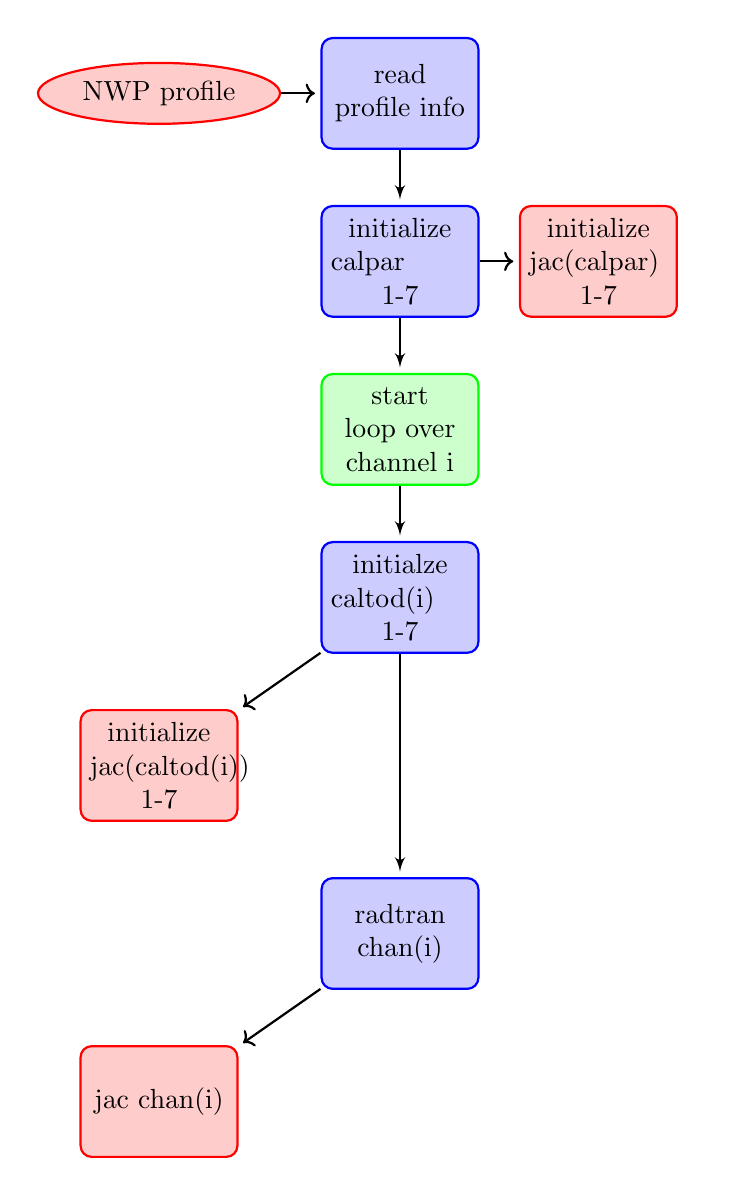
\begin{tikzpicture}
[auto,
decision/.style={diamond, draw=blue, thick, fill=blue!20,
text width=4.5em,align=flush center,
inner sep=1pt},
block/.style ={rectangle, draw=blue, thick, fill=blue!20,
text width=5em,align=center, rounded corners,
minimum height=4em},
block2/.style ={rectangle, draw=red, thick, fill=red!20,
text width=5em,align=center, rounded corners,
minimum height=4em},
blockG/.style ={rectangle, draw=green, thick, fill=green!20,
text width=5em,align=center, rounded corners,
minimum height=4em},
line/.style ={draw, thick, -latex',shorten >=2pt},
cloud/.style ={draw=red, thick, ellipse,fill=red!20,
minimum height=2em}]
\matrix [column sep=5mm,row sep=7mm]
{
% row 1  has three thingies
\node [cloud]  (nwp)  {NWP profile}; &
\node [block] (init) {read profile info}; & \\
% row 2 has a blank thingy and another thingy and a blank thigy
& \node [block]  (calpar)    {initialize calpar \newline 1-7}; & 
  \node [block2] (calparjac) {initialize jac(calpar) \newline 1-7}; \\
% row 3
& \node [blockG] (loop)       {start loop over channel i}; & & \\
% row 4
& \node [block] (caltod)     {initialze caltod(i) \newline 1-7}; & \\
  \node [block2] (caltodjac) {initialize jac(caltod(i)) \newline 1-7};  \\
% row 5
& \node [block] (radtrans)     {radtran chan(i)}; & \\
  \node [block2] (radtransjac) {jac chan(i)};  \\
};
\begin{scope}[every path/.style=line]
\path [->] (nwp) -- (init);
\path      (init) -- (calpar);
\path      (calpar) -- (loop);
\path [->] (calpar) -- (calparjac);
\path      (caltod) -- (radtrans);
\path      (loop) --   (caltod);
\path [->] (caltod) -- (caltodjac);
\path [->] (radtrans) -- (radtransjac);
\end{scope}
\end{tikzpicture}

\end{document} 
